\section{Experimental results\textsuperscript{2}}
For a proof-of-concept implementation of the proposed architecture, we implemented the management of a coffee vending machine (Figure \ref{fig:coffeemachine}) at the computer science faculty at the Bielefeld University of Applied Sciences (Campus Minden).
\begin{figure}[ht]
    \centering
    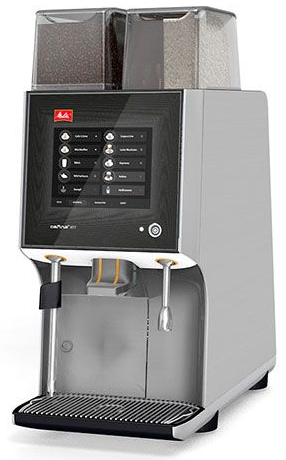
\includegraphics[width=0.3\textwidth]{assets/cafina-xt7.png}
    \caption{Melitta Cafina XT7 coffee machine}
    \label{fig:coffeemachine}
\end{figure}
In this implementation, a Raspberry Pi is physically located next to the coffee machine and is connected to the machines RS232 serial port, which provides the Coffee Credit Interface (CCI) \cite{csi:online} and is intended for external payment devices, like banknote or coin counters.
The Raspberry Pi has internet access and additionally provides a Bluetooth module by which customers can identify themself for payment of various coffee products.
The Raspberry Pi, the customer mobile app and the management application for all stakeholders connect to the cloud-based Hyperledger Fabric instance, were vending machine, settings and account balances are stored. Additionally a fake payment provider is implemented in order to deposit credits without actually making payments.

For evaluation of the proposed architecture, we compare the implemented proof-of-concept with the requirements defined in the Methods section.
Because the proof-of-concept is built using a permissioned blockchain approach, interaction with the entire system is possible without paying transaction fees. With that, the management of vending machines, or in this case the coffee machine, also does not generate costs. The distributed ledger, which is shared between all stakeholders ensures transparency of transaction history and avoids manipulation by any participant of the network.

\begin{figure}[ht]
    \centering
    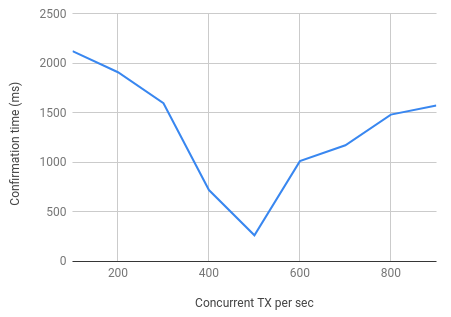
\includegraphics[width=0.5\textwidth]{assets/benchmark.png}
    \caption{Concurrent transactions benchmark}
    \label{fig:benchmark}
\end{figure}
For further evaluation, we benchmarked the transaction throughput of the proposed architecture. Figure \ref{fig:benchmark} shows the lowest confirmation time of around 250 milliseconds at 500 transactions per second, which matches with the configured blocksize of 500 transactions. This value marks the lowest confirmation time, because a new block is instantly filled. Lower and higher transaction-per-second values result in higher confirmation times, which are still acceptable. In these cases the maximum blocktime is triggered at which point a block is finalized. These values fulfill the essential requirement of the system regarding transaction speed and are even lower than EC payment transaction speed.
With the payment provider interface, the system allows the future integration or replacement of payment providers. 
Regarding the user experience requirements, the use of common smartphones, Bluetooth technology and a simple payment application ensures low barriers for interaction with the system for customers. The statistics and configuration capability provided by the management application allows insight into sales figures and enables stakeholder to make strategic decisions about vending machine deployment.
